\section{Reversibilidade regularizada e ponte quantitativa com redes ReLU}
\label{sec:regularized-reversibility}

Uma função linear por partes pode ser representada exatamente por uma rede ReLU
rasa por meio de uma expansão em hinges
\citep{devorehaninpetrova2021,daubechies2022}. Ela pode, portanto, ter poucas
folhas e, por isso, ter erro bruto nulo em todas as escalas posteriores sem
ganhar suavidade clássica. Essa barreira determina a forma dos teoremas
inversos desta seção.

Há três respostas, em níveis diferentes. Primeiro, o erro bruto admite uma
imersão inversa com perda, desde que se controle a inclinação efetivamente
realizada pelos aproximantes. Segundo, uma extensão marcada da biblioteca
remove a obstrução das regiões planas e dá uma equivalência exata com redes
ReLU rasas racionais de quebras diádicas; redes reais genéricas admitem uma
volta aproximada com recursos explícitos. Terceiro, usa-se um funcional de
realização, no sentido clássico de \citet{hristovivanov1990}, que soma ao erro
a autorregularidade do próprio aproximante. Nesse terceiro nível, a
desigualdade inversa é universal; a contribuição específica da biblioteca é o
lado direto de Jackson sob uma agenda explícita de altura racional.

A necessidade de orçar o crescimento dos coeficientes e a profundidade em
espaços de aproximação neural é enfatizada em
\citet{gribonval2022,grohs2023,guhringraslan2021}. Em particular, o expoente crítico de Hölder
que surgirá no \cref{thm:raw-lossy-inverse} é a contraparte unidimensional e
uniforme do mecanismo de imersão de \citet{grohs2023}. As provas abaixo usam
apenas os módulos de suavidade e a altura da biblioteca.

\subsection{A obstrução que toda volta deve respeitar}

Escreva
\begin{equation}
 \psi(x)=\left|x-\frac12\right|,
 \qquad x\in[0,1].
 \label{eq:reverse-kink}
\end{equation}
Ela é uma montagem de duas folhas e altura $4$. Logo, para toda agenda que
eventualmente satisfaz $H(N)\ge4$,
\begin{equation}
 e_N^{\Library,H}(\psi)=0
 \quad\text{para todo $N$ suficientemente grande},
 \qquad
 \psi\in\mathscr A_q^\alpha(\Library,H)
 \quad(\alpha>0,\ 0<q\le\infty).
 \label{eq:kink-zero-raw-error}
\end{equation}
Por outro lado,
\begin{equation}
 \omega_2(\psi,h)_{\infty,[0,1]}=2h,
 \qquad 0<h\le\frac12,
 \label{eq:kink-exact-modulus-reverse}
\end{equation}
e, portanto,
\begin{equation}
 \psi\in B^s_{\infty,q}([0,1])
 \quad\Longleftrightarrow\quad
 s<1\ \text{ ou }\ (s=1\text{ e }q=\infty),
 \qquad 0<s<2.
 \label{eq:kink-besov-reverse}
\end{equation}
Com efeito, o salto de inclinação de $\psi$ é $2$, logo toda segunda diferença
de passo $h$ tem módulo no máximo $2h$; nos pontos
$1/2-h,1/2,1/2+h$ ela tem módulo exatamente $2h$. Substituir essa identidade
na caracterização diádica \eqref{eq:dyadic-besov-norm} prova
\eqref{eq:kink-besov-reverse}. Em particular, nenhum
teorema da forma
\begin{equation}
 e_N(f)=O(N^{-\alpha})\quad\Longrightarrow\quad
 f\in B^s_{\infty,q},
 \qquad s>1,
 \label{eq:forbidden-unregularized-converse}
\end{equation}
pode valer para o erro bruto do catálogo. Uma versão reversível deve conservar
informação sobre as quinas do aproximante, e não apenas sobre a distância de
$f$ a ele.

\subsection{A extensão marcada e a volta ReLU exata}

A primeira limitação é combinatória, não analítica. A inclinação nula foi
excluída da biblioteca original porque a imagem de um segmento constante não
recupera o suporte. Para estudar a volta, introduzimos uma extensão auxiliar
que guarda esse suporte como parte do código.

\begin{definition}[biblioteca marcada completa]
\label{def:marked-completion}
A biblioteca $\Library^\square$ é formada pelas quádruplas marcadas
\begin{equation}
 (k,m,y_0,s)\in\Nzero\times\mathbb Z\times\mathbb Q\times\mathbb Q,
 \label{eq:marked-atoms}
\end{equation}
com o mesmo segmento \eqref{eq:inherited-atom} e a mesma altura
\eqref{eq:inherited-height}. A marca $(k,m)$ é conservada na decodificação,
inclusive quando $s=0$. Denote por $\Aclass^\square(K)$ suas montagens
contínuas e por $\Aclass^\square_{N,H}(K)$ aquelas com no máximo $N$
folhas e altura atômica no máximo $H$.
\end{definition}

Tem-se $\Library\subset\Library^\square$. Para $s\ne0$, a marca é redundante
e a recuperação pela imagem coincide com a de $\Library$; para $s=0$, o
suporte é conservado explicitamente no par $(k,m)$.

Considere a forma ReLU reduzida
\begin{equation}
 R(x)=c+qx+\sum_{j=1}^{M}a_j\rho(x-\tau_j),
 \qquad 0<\tau_1<\cdots<\tau_M<1,
 \qquad a_j\ne0,
 \label{eq:reduced-relu-reverse}
\end{equation}
e suas inclinações locais
\begin{equation}
 \sigma_i=q+\sum_{j=1}^{i}a_j,
 \qquad 0\le i\le M.
 \label{eq:reverse-local-slopes}
\end{equation}
Para um conjunto finito $S\subset\mathbb D\cap(0,1)$, seja
$\mathcal T(S)$ a árvore diádica menos refinada cujas folhas não contêm
pontos de $S$ no interior. Ela é obtida subdividindo exatamente os ancestrais
necessários para transformar cada ponto de $S$ em fronteira.

\begin{theorem}[reversibilidade rasa exata]
\label{thm:exact-marked-reversal}
Uma função na forma reduzida \eqref{eq:reduced-relu-reverse} pertence a
$\Aclass^\square([0,1])$ se e somente se
\begin{equation}
 c,q,a_1,\ldots,a_M\in\mathbb Q,
 \qquad
 \tau_1,\ldots,\tau_M\in\mathbb D.
 \label{eq:marked-reversal-conditions}
\end{equation}
Nessas condições, $\mathcal T(\{\tau_1,\ldots,\tau_M\})$ é a única árvore
menos refinada que realiza $R$. Se $N_{\rm can}(R)$ é seu número de folhas e
$d_j$ é a profundidade diádica reduzida de $\tau_j$, então
\begin{equation}
 M+1\le N_{\rm can}(R)
 \le 1+\sum_{j=1}^{M}d_j.
 \label{eq:canonical-tree-leaf-bounds}
\end{equation}
A função pertence à biblioteca original $\Aclass([0,1])$ exatamente quando,
além de \eqref{eq:marked-reversal-conditions},
\begin{equation}
 \sigma_i\ne0\qquad(0\le i\le M).
 \label{eq:original-nonflat-condition}
\end{equation}
\end{theorem}

\begin{proof}
Suponha \eqref{eq:marked-reversal-conditions}. A árvore canônica transforma
todas as quebras em fronteiras. Em cada folha $J$, a função $R$ é afim, sua
inclinação é uma das $\sigma_i\in\mathbb Q$ e seu valor no centro é racional.
Esses dados determinam um átomo marcado; a continuidade de $R$ cola as peças.

Reciprocamente, toda montagem marcada é racional e afim no interior de cada
folha. Toda quebra real está em uma fronteira diádica, seu valor em $0$, a
inclinação inicial e os saltos de inclinação são racionais. Pela unicidade da
forma reduzida, obtém-se \eqref{eq:marked-reversal-conditions}.

Qualquer árvore que realize $R$ deve separar suas $M$ quebras reais, logo tem
ao menos $M+1$ folhas e refina $\mathcal T(S)$. Para inserir uma quebra de
profundidade $d_j$, bastam no máximo $d_j$ subdivisões novas. Como cada
subdivisão acrescenta uma folha, resulta a cota superior em
\eqref{eq:canonical-tree-leaf-bounds}. Finalmente, um átomo da biblioteca
original possui inclinação não nula; a condição é também suficiente folha a
folha.
\end{proof}

O teorema distingue duas contagens que coincidem apenas em partições já
alinhadas. $M+1$ conta regiões afins máximas; $N_{\rm can}$ conta células
diádicas. Por exemplo, uma única quebra em $1/4$ produz duas regiões, mas a
região $[1/4,1]$ precisa de duas folhas diádicas.

\begin{definition}[altura canônica de rede]
\label{def:canonical-network-height}
Para uma rede que satisfaz \eqref{eq:marked-reversal-conditions}, defina
\begin{equation}
 H_{\rm can}(R)=
 \max_{J_{k,m}\in\operatorname{leaf}(\mathcal T(S))}
 \max\{2,k+1,|m|+1,\height(R(x_{k,m})),\height(R'|_{J_{k,m}})\}.
 \label{eq:canonical-network-height}
\end{equation}
\end{definition}

Por construção, $H_{\rm can}(R)$ é exatamente a maior altura dos átomos na
montagem canônica. Essa é a medida que torna a ida e a volta isométricas no
recurso aritmético. A altura ingênua dos coeficientes
$(c,q,a_1,\ldots,a_M)$ não tem essa propriedade: somas de racionais podem
multiplicar denominadores.

\begin{proposition}[forma ancorada e comprimento estrutural]
\label{prop:anchored-relu-code}
Se $g\in\Aclass^\square_{N,H}([0,1])$, sua forma reduzida possui
$M\le N-1$ hinges e pode ser escrita, tomando o centro $x_*$ da folha mais à
esquerda, como
\begin{equation}
 g(x)=g(x_*)+\sigma_0(x-x_*)
      +\sum_{j=1}^{M}(\sigma_j-\sigma_{j-1})\rho(x-\tau_j).
 \label{eq:anchored-relu-form}
\end{equation}
Os valores $g(x_*)$ e $\sigma_i$ têm altura no máximo $H$, os saltos têm
altura no máximo $2H^2$, e os pontos diádicos são transmitidos por seus pares
estruturais. Consequentemente, existe uma codificação prefix-free da forma
ancorada com
\begin{equation}
 L_{\rm ReLU}^{\rm anc}(g)=O(N\log(2H)).
 \label{eq:anchored-network-bits}
\end{equation}

Na direção contrária, se os coeficientes de
\eqref{eq:reduced-relu-reverse} têm altura no máximo $W$ e as quebras têm
profundidade no máximo $D$, então
\begin{equation}
 \log_2 H_{\rm can}(R)
 \le C\bigl[M\log(2W)+D+\log(M+1)\bigr]
 \label{eq:reverse-height-bit-bound}
\end{equation}
para uma constante universal $C$.
\end{proposition}

\begin{proof}
Na ida, cada salto é a diferença de duas inclinações de altura no máximo
$H$, logo sua altura não excede $2H^2$. A altura atômica limita os inteiros
estruturais da célula, e todos os campos usam $O(\log(2H))$ bits. Somar os
$O(N)$ campos prova \eqref{eq:anchored-network-bits}. O ancoramento evita
expandir desnecessariamente $g(x_*)-\sigma_0x_*$ em um intercepto com
denominador diádico explícito.

Na volta, cada inclinação local é soma de no máximo $M+1$ racionais. Um
denominador comum tem no máximo $O(M\log(2W))$ bits. Avaliar em um centro de
profundidade no máximo $D$ acrescenta $D+O(\log(M+1))$ bits. Exponenciar a
cota de comprimento fornece \eqref{eq:reverse-height-bit-bound}.
\end{proof}

Assim, a reversibilidade exata preserva comprimento binário em ordem
polinomial, mas não preserva a altura ingênua coeficiente a coeficiente. A
altura correta do lado neural é \eqref{eq:canonical-network-height}, isto é,
o recurso aritmético depois da função ser colocada em sua partição diádica
canônica.

\subsection{Volta aproximada para redes rasas reais}

Quebras não diádicas e coeficientes irracionais impedem igualdade exata, mas
não uma conversão quantitativa. Cotas de erro e de recursos para aproximação
ReLU, inclusive sob restrições de codificação, são estudadas em
\citet{yarotsky2017,bolcskei2019}. A próxima estimativa dá uma forma explícita
da densidade compatível com a biblioteca.

\begin{theorem}[reversão aproximada quantizada]
\label{thm:quantized-approximate-reverse}
Seja $R$ como em \eqref{eq:reduced-relu-reverse}, agora com parâmetros reais,
e suponha
\begin{equation}
 |c|,|q|,|a_1|,\ldots,|a_M|\le W,
 \qquad W\ge1.
 \label{eq:real-network-weight-bound}
\end{equation}
Para todo $0<\varepsilon\le1$, existe uma montagem da biblioteca original
$g_\varepsilon\in\Aclass([0,1])$ tal que
\begin{align}
 \|R-g_\varepsilon\|_\infty&\le\varepsilon,
 \label{eq:approximate-reverse-error}\\
 |\Lambda(g_\varepsilon)|&\le1+MD_\varepsilon,
 \qquad
 D_\varepsilon=
 \left\lceil\log_2\frac{C(M+1)(W+1)}{\varepsilon}\right\rceil,
 \label{eq:approximate-reverse-leaves}\\
 \height_{\max}(g_\varepsilon)
 &\le
 C(M+1)^3(W+1)^3\varepsilon^{-2},
 \label{eq:approximate-reverse-height}
\end{align}
onde $C$ é universal. A conclusão permanece válida quando $R$ possui regiões
planas.
\end{theorem}

\begin{proof}
Ponha
\[
 \delta=\frac{\varepsilon}{16(M+1)(W+1)}.
\]
Escolha um denominador comum $Q\asymp\delta^{-1}$ e aproxime
$c,q,a_1,\ldots,a_M$ por múltiplos de $1/Q$ com erro no máximo $\delta$.
Aproxime cada $\tau_j$ por um diádico de profundidade
$D\le D_\varepsilon$. A função $z\mapsto\rho(x-z)$ é $1$-Lipschitz e
$0\le\rho(x-z)\le1$ em $[0,1]$, de modo que a soma dos erros de coeficientes
e deslocamentos é no máximo
\[
 (M+2)\delta+M(W+\delta)\delta.
\]
Nós que colidem são combinados; nós que chegam a $0$ são absorvidos no termo
linear e os que chegam a $1$ desaparecem no domínio.

Resta impedir inclinações locais nulas. Depois da quantização há no máximo
$M+1$ valores proibidos para uma perturbação global da inclinação. Entre
$M+2$ múltiplos positivos consecutivos de $1/Q$, escolha um que não seja
proibido e acrescente o termo correspondente $\eta x$. A escolha de $Q$ e a
folga em $\delta$ mantêm o erro total abaixo de $\varepsilon$.

A árvore canônica exige no máximo $1+MD$ folhas pelo
\cref{thm:exact-marked-reversal}. Inclinações locais têm denominador comum
$Q$ e numeradores $O((M+1)(W+1)Q)$. Valores nos centros têm denominador que
divide $Q2^{D+1}$ e numeradores
$O((M+1)(W+1)Q2^D)$. Como
$Q,2^D=O((M+1)(W+1)\varepsilon^{-1})$, segue
\eqref{eq:approximate-reverse-height}. A perturbação final permite usar a
biblioteca original, não apenas sua extensão marcada.
\end{proof}

\begin{corollary}[redes profundas medidas pela função realizada]
\label{cor:deep-functional-reverse}
Se uma rede ReLU univariada arbitrária realiza uma função $F$ com $R(F)$
regiões afins máximas, norma uniforme no máximo $B$ e constante de Lipschitz
no máximo $L_F$, então o \cref{thm:quantized-approximate-reverse} vale com
\begin{equation}
 M=R(F)-1,
 \qquad
 W\le2\max\{1,B,L_F\}.
 \label{eq:deep-realized-resources}
\end{equation}
\end{corollary}

\begin{proof}
Toda função ReLU univariada é linear por partes e admite a forma hinge rasa
canônica, independentemente da arquitetura que a produziu. A inclinação
inicial tem módulo no máximo $L_F$, cada salto tem módulo no máximo $2L_F$ e
$|F(0)|\le B$. Aplique o teorema anterior.
\end{proof}

A relação entre profundidade e número de regiões pode ser exponencial, como nas
construções de separação por profundidade de \citet{telgarsky2016}. Para o bloco
tenda
\[
 T(x)=2\rho(x)-4\rho(x-\tfrac12),\qquad x\in[0,1],
\]
a iterada $T_L=T^{\circ L}$ possui exatamente $2^L$ regiões afins máximas,
com inclinações $\pm2^L$: cada composição bissecta todas as regiões do nível
anterior. Assim, toda montagem que realize $T_L$ exatamente requer ao menos
$2^L$ folhas e altura atômica ao menos $2^L$. A dependência do corolário nos
recursos realizados conserva, portanto, essa separação exponencial.

A \cref{tab:deep-tent-network} explicita os primeiros oito níveis dessa lei,
e a \cref{fig:network-restrictions} contrasta número de blocos, regiões
realizadas e recursos mínimos da biblioteca.

\begin{table}[t]
 \centering
 \small
 \begin{tabular}{rrrr}
\toprule
profundidade $L$ & blocos & regiões/folhas mín. & altura mín.\\
\midrule
1 & 1 & 2 & 2\\
2 & 2 & 4 & 4\\
3 & 3 & 8 & 8\\
4 & 4 & 16 & 16\\
5 & 5 & 32 & 32\\
6 & 6 & 64 & 64\\
7 & 7 & 128 & 128\\
8 & 8 & 256 & 256\\
\bottomrule
\end{tabular}

 \caption{Separação exata para a tenda iterada: $L$ blocos produzem $2^L$
 regiões, e qualquer montagem exata requer ao menos $2^L$ folhas e altura
 atômica ao menos $2^L$.}
 \label{tab:deep-tent-network}
\end{table}

\begin{figure}[t]
 \centering
 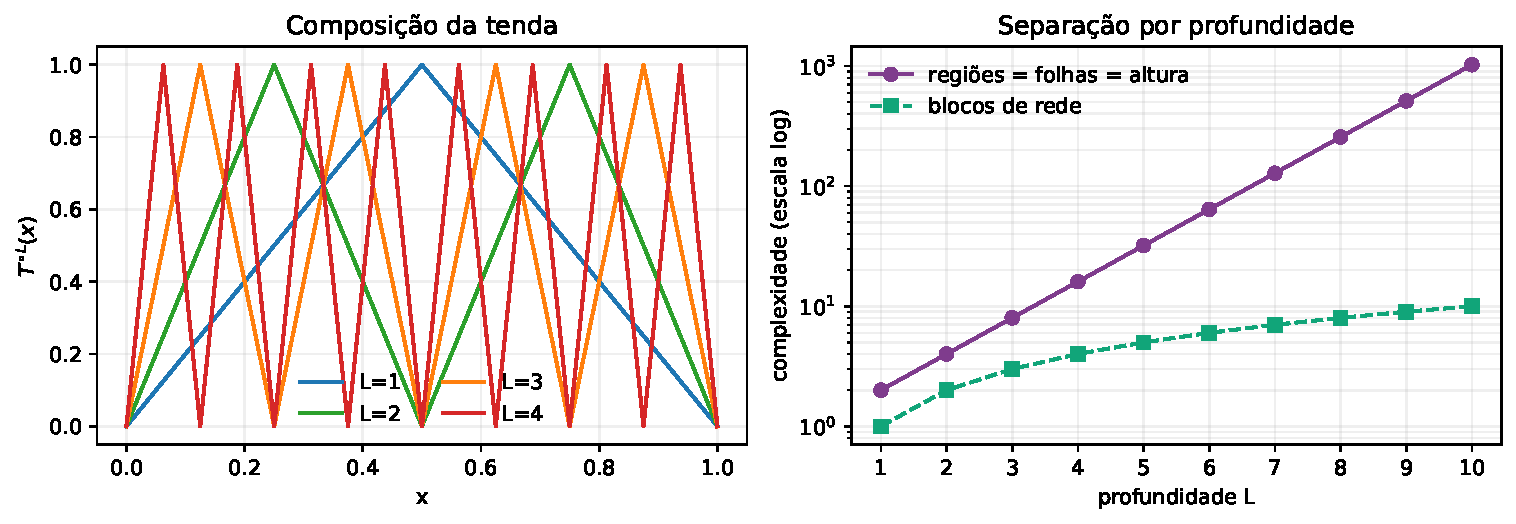
\includegraphics[width=.88\linewidth]{fig_restricoes_rede.pdf}
 \caption{Crescimento dos recursos realizados pela tenda iterada. Os pontos
 provêm de identidades exatas; as linhas apenas guiam a leitura.}
 \label{fig:network-restrictions}
\end{figure}

\begin{table}[t]
 \centering
 \small
 \begin{tabular}{rrrrrr}
\toprule
$M$ & $\varepsilon$ & $D$ & folhas & cota de folhas & erro/$\varepsilon$\\
\midrule
1 & $1/32$ & 12 & 13 & 13 & 0.0099\\
1 & $1/64$ & 13 & 14 & 14 & 0.0037\\
1 & $1/128$ & 14 & 15 & 15 & 0.0131\\
1 & $1/32$ & 11 & 12 & 12 & 0.0245\\
1 & $1/64$ & 12 & 13 & 13 & 0.0099\\
1 & $1/128$ & 13 & 14 & 14 & 0.0120\\
\bottomrule
\end{tabular}

 \caption{Primeiras seis testemunhas da bateria racional de reversão
 aproximada. As redes de entrada possuem quebras não diádicas. O erro é
 calculado exatamente no conjunto unido de quebras, onde o máximo de uma
 diferença linear por partes é atingido; a última coluna arredonda a quatro
 casas as razões exatas do arquivo suplementar.}
 \label{tab:approximate-reverse-audit}
\end{table}

A bateria suplementar fixa $c=1/5$, escolhe de uma a três quebras entre
$\{1/3,2/5,5/7\}$, toma a inclinação inicial em
$(-7/3,-1/2,2/3,5/4)$ e, para $M$ quebras, usa saltos
$a_i=b_{(i+M)\bmod4}$, onde
$(b_0,b_1,b_2,b_3)=(-7/3,-1/2,2/3,5/4)$. Para cada rede são usados
$\varepsilon\in\{1/32,1/64,1/128\}$, totalizando $84$ quantizações. As redes
de entrada, as frações brutas e as razões exatas das seis linhas exibidas
ficam em \path{reproducibility/selecao/resultados_reversibilidade.json}.
Assim, a \cref{tab:approximate-reverse-audit} apresenta testemunhas
reprodutíveis, e não vetores de teste implícitos.

\subsection{A melhor recíproca para o erro bruto}

Todo $g\in\Sigma_N^{\Library,H}$ é $H(N)$-Lipschitz, pois em cada folha sua
inclinação $s$ satisfaz $|s|\le\height(s)\le H(N)$. Consequentemente,
$\omega_2(g,t)_\infty\le2H(N)t$. Essa desigualdade de tipo Bernstein contém
uma recíproca verdadeira, desde que se aceite a perda imposta pelo crescimento
das inclinações. A formulação seguinte não depende da aritmética.

\begin{theorem}[imersão inversa sob crescimento de Lipschitz]
\label{thm:raw-lossy-inverse}
Sejam $\mathcal G_N\subset C([0,1])$ famílias de aproximantes tais que
\begin{equation}
 \operatorname{Lip}(g)\le C_LN^\gamma
 \qquad(g\in\mathcal G_N),
 \qquad \gamma\ge0,
 \label{eq:lipschitz-growth-family}
\end{equation}
e defina
$e_N^{\mathcal G}(f)=\inf_{g\in\mathcal G_N}\|f-g\|_\infty$. Se
\begin{equation}
 A_\alpha(f):=\sup_{N\ge1}N^\alpha e_N^{\mathcal G}(f)<\infty,
 \qquad \alpha>0,
 \label{eq:raw-rate-assumption}
\end{equation}
então, com
\begin{equation}
 \theta_* = \frac{\alpha}{\alpha+\gamma},
 \label{eq:critical-reverse-exponent}
\end{equation}
vale
\begin{equation}
 \omega_2(f,t)_\infty
 \le C_{\alpha,\gamma}(A_\alpha(f)+C_L)t^{\theta_*},
 \qquad 0<t\le\frac12.
 \label{eq:raw-inverse-modulus}
\end{equation}
Consequentemente,
\begin{equation}
 f\in B^{\theta_*}_{\infty,\infty}([0,1])
 \quad\text{e}\quad
 f\in B^\theta_{\infty,r}([0,1])
 \quad(0<\theta<\theta_*,\ 0<r\le\infty).
 \label{eq:raw-inverse-besov}
\end{equation}
\end{theorem}

\begin{proof}
Para qualquer $g\in\mathcal G_N$, a desigualdade triangular para segundas
diferenças e a propriedade Lipschitz dão
\begin{equation}
 \omega_2(f,t)_\infty
 \le4\|f-g\|_\infty+2C_LN^\gamma t.
 \label{eq:inverse-balance}
\end{equation}
Escolha $N$ comparável a $t^{-1/(\alpha+\gamma)}$ e use um aproximante
arbitrariamente próximo do ínfimo. Os dois termos do lado direito passam a
ser $O(t^{\alpha/(\alpha+\gamma)})$, o que prova
\eqref{eq:raw-inverse-modulus}. A caracterização diádica de Besov fornece o
endpoint por supremo. Para $\theta<\theta_*$, a sequência normalizada ganha o
fator geométrico $2^{-j(\theta_*-\theta)}$ e pertence a todo $\ell^r$.
\end{proof}

\begin{corollary}[aplicação às agendas diretas]
\label{cor:raw-library-inverse}
Se $H(N)\le C N^\gamma$, então
\begin{equation}
 \mathscr A_q^\alpha(\Library,H)
 \subset B^{\alpha/(\alpha+\gamma)}_{\infty,\infty}([0,1]),
 \qquad 0<q\le\infty.
 \label{eq:raw-library-inverse}
\end{equation}
Para as agendas $H_{s,0}$ da \cref{sec:direct-height}, isso dá
\begin{equation}
 \mathscr A_q^s(\Library,H_{s,0})
 \subset B^{\vartheta_s}_{\infty,\infty},
 \qquad
 \vartheta_s=
 \begin{cases}
 s/(s+1),&0<s<1,\\
 1/2,&1\le s<2.
 \end{cases}
 \label{eq:corrected-schedule-raw-inverse}
\end{equation}
Se a agenda possui ainda um fator logarítmico, a mesma conclusão vale para
toda ordem estritamente menor que $\vartheta_s$.
\end{corollary}

\begin{proof}
Todo elemento de $\Sigma_N^{\Library,H}$ é $H(N)$-Lipschitz. O funcional com
$q<\infty$ controla o de supremo pela redução diádica do
\cref{thm:dyadic-rate-equivalence}. Um fator logarítmico é dominado por
$N^\eta$ para qualquer $\eta>0$; aplique o teorema com
$\gamma+\eta$ e faça $\eta\downarrow0$.
\end{proof}

O expoente \eqref{eq:critical-reverse-exponent} não é uma folga do balanço.
O \cref{thm:critical-tent-comb} transfere a testemunha para a biblioteca
original, inclusive com a exigência de inclinações locais não nulas.

\begin{theorem}[agudeza por um pente de tendas]
\label{thm:critical-tent-comb}
Fixe $0<\alpha\le\gamma$ e ponha
$\theta_*=\alpha/(\alpha+\gamma)$. Existe
$f\in C([0,1])$ e uma constante $C$ tais que, para a biblioteca original sob
$H(N)=\lceil CN^\gamma\rceil$,
\begin{equation}
 e_N^{\Library,H}(f)\le CN^{-\alpha},
 \label{eq:comb-approximation-rate}
\end{equation}
mas
\begin{equation}
 f\notin B^\theta_{\infty,\infty}\quad(\theta>\theta_*),
 \qquad
 f\notin B^{\theta_*}_{\infty,r}\quad(0<r<\infty).
 \label{eq:comb-sharpness}
\end{equation}
\end{theorem}

\begin{proof}
Escolha um inteiro $J_0$ tão grande que
$J_0(\alpha+\gamma)>3$. Para $j\ge1$, ponha
\[
 a_j=\lceil J_0\alpha j\rceil,
 \qquad b_j=\lfloor J_0\gamma j\rfloor,
 \qquad r_j=a_j+b_j-1.
\]
No intervalo diádico $J_{r_j,1}$, coloque uma tenda $\phi_j$ de altura
$2^{-a_j}$, nula nas extremidades e linear em cada metade. As escolhas
garantem que os suportes são disjuntos e acumulam apenas em $0$. Defina
$f=\sum_{j\ge1}\phi_j$.

A inclinação da $j$-ésima tenda tem módulo $2^{b_j}$ e os valores centrais de
suas duas metades têm altura $2^{a_j+1}$. Seja $T_j$ a árvore diádica em pente
que isola as duas metades das primeiras $j$ tendas. Ela possui
$O(r_j+j)$ folhas; fora dessas tendas, a soma parcial
$f_j=\sum_{i\le j}\phi_i$ é nula em cada folha restante.

Para eliminar todas as inclinações nulas sem alterar o alvo $f$, subdivida uma
vez cada folha plana $J$ de $T_j$ e, sobre $J$, acrescente uma tenda
$\psi_{J,j}$ nula nos extremos e de altura
\[
 \delta_j=2^{-a_{j+1}-2}
\]
no ponto médio. Os suportes dessas pequenas tendas são disjuntos. A função
\[
 g_j=f_j+\sum_{J\ {\rm plano\ em}\ T_j}\psi_{J,j}
\]
é contínua e tem inclinação não nula em toda folha da árvore refinada. Logo
$g_j$ é uma montagem da biblioteca original, não da extensão marcada.

Resta conferir os dois orçamentos. A árvore refinada tem ainda
$O(r_j+j)$ folhas. Em uma folha plana de profundidade $d\le r_j+1$, a nova
inclinação tem módulo $2^{d+1}\delta_j$; sua altura é limitada por
\[
 \max\{2^{a_{j+1}+1},\,2^{r_j-a_{j+1}}\}
 \le C2^{J_0\gamma j}.
\]
Os valores centrais novos têm altura no máximo $2^{a_{j+1}+3}$, e os
parâmetros das tendas originais são limitados por
$C\max\{2^{a_j},2^{b_j}\}$. As células profundas do pente têm índices
$m\in\{0,1,2,3\}$; portanto escala e translação obedecem à mesma cota.
Como $\alpha\le\gamma$, todos esses termos são no máximo
$CN_j^\gamma$ para $N_j=2^{J_0j}$, depois de aumentar $C$. Também
$O(r_j+j)\le N_j$ para $j$ grande; as finitíssimas escalas iniciais são
absorvidas em $C$ e por uma reindexação finita.

Por disjunção dos suportes,
\[
 \|f-g_j\|_\infty
 \le \Bigl\|\sum_{i>j}\phi_i\Bigr\|_\infty+\delta_j
 \le 2^{-a_{j+1}}+\delta_j
 \le C N_j^{-\alpha}.
\]
Para $N_j\le N<N_{j+1}$, use $g_j$; a razão
$N_{j+1}/N_j=2^{J_0}$ é fixa. A monotonicidade da agenda e o ajuste dessa
constante provam \eqref{eq:comb-approximation-rate} para todo $N$.

Se $h_j=2^{-(r_j+1)}$ é a meia-largura da tenda, os valores
$0,2^{-a_j},0$ dão
\[
 \omega_2(f,h_j)_\infty\ge2^{1-a_j}\asymp h_j^{\theta_*}.
\]
Isso exclui toda ordem maior no supremo e torna constante uma subsequência do
coeficiente crítico, que não pertence a nenhum $\ell^r$ finito.
\end{proof}

A exigência $\alpha\le\gamma$ cobre em particular as agendas críticas da
\cref{sec:direct-height}. Ela também expõe por que a informação correta é a inclinação
realizada, não a altura do endereço isoladamente.

\subsection{Funcional de realização: lado direto com altura controlada}

A agudeza do teorema anterior fixa a regularidade determinada pelo erro bruto
e por uma cota de Lipschitz. Para comparar com a suavidade clássica, considere
o funcional de realização associado ao módulo de segunda ordem. Funcionais
desse tipo foram introduzidos para substituir $K$-funcionais degenerados em
aproximação restrita \citep{hristovivanov1990}. Para $N\ge2$, defina
\begin{equation}
 \mathcal R_N^{\Library,H}(f)
 :=\inf_{g\in\Sigma_N^{\Library,H}([0,1])}
 \left\{\|f-g\|_\infty+
 \omega_2(g,N^{-1})_\infty\right\}.
 \label{eq:self-roughness-certificate}
\end{equation}
O primeiro termo mede fidelidade; o segundo impede que uma função com quinas
receba suavidade apenas porque já pertence ao catálogo.

\begin{lemma}[desigualdade inversa universal]
\label{lem:universal-regularized-inverse}
Para toda agenda, toda $f\in C([0,1])$ e todo $N\ge2$,
\begin{equation}
 \frac14\omega_2(f,N^{-1})_\infty
 \le \mathcal R_N^{\Library,H}(f).
 \label{eq:universal-regularized-lower}
\end{equation}
\end{lemma}

\begin{proof}
Para qualquer $g$ admissível,
\[
 \omega_2(f,N^{-1})_\infty
 \le4\|f-g\|_\infty+\omega_2(g,N^{-1})_\infty
 \le4\bigl(\|f-g\|_\infty+\omega_2(g,N^{-1})_\infty\bigr).
\]
Tome o ínfimo.
\end{proof}

\begin{remark}[o que o funcional mede]
\label{rem:realization-functional-scope}
A prova do \cref{lem:universal-regularized-inverse} usa apenas a desigualdade
triangular para segundas diferenças; não usa racionalidade, células diádicas,
altura nem sequer linearidade por partes. Portanto, a direção inversa mede a
suavidade do alvo e vale para qualquer família de candidatos. Ela não é uma
medida específica de aproximabilidade pela biblioteca. O conteúdo específico
deste trabalho é o lado direto: construir, dentro de $\Library$, candidatos
que atingem o majorante com a agenda aritmética explicitada na
\cref{sec:direct-height}.
\end{remark}

\begin{theorem}[Jackson racional para o funcional de realização]
\label{thm:regularized-jackson-bernstein}
Se $0<s<2$ e $f\in B^s_{\infty,\infty}([0,1])$, então, para toda potência de
dois $N$ suficientemente grande e toda altura que satisfaz as hipóteses do
\cref{lem:rational-jackson-height},
\begin{equation}
 \frac14\omega_2(f,N^{-1})_\infty
 \le \mathcal R_N^{\Library,H}(f)
 \le C_0\omega_2(f,N^{-1})_\infty+\frac{C_f}{H(N)},
 \label{eq:two-sided-regularized-equivalence}
\end{equation}
onde $C_0$ é universal e $C_f$ depende apenas de $\|f\|_\infty$ e das
constantes fixadas na racionalização.
Se $\|f\|_{B^s_{\infty,\infty}}^*\le B$, $B\ge1$, e
$H(N)\ge\widehat H_{s,0}^{[B]}(N)$, a mesma estimativa vale para toda potência
diádica $N\ge2$, com $C_f/H(N)$ substituído por $C(B+1)/H(N)$ e constantes
independentes de $f$.
\end{theorem}

\begin{proof}
A cota inferior é o lema anterior. Para a superior, tome o aproximante
racional $g_{N,H}$ do \cref{lem:rational-jackson-height}. Ele satisfaz
\[
 \|f-g_{N,H}\|_\infty
 \le2C_W\omega_2(f,N^{-1})_\infty+C_fH(N)^{-1}.
\]
Além disso, a desigualdade triangular aplicada na direção contrária dá
\[
 \omega_2(g_{N,H},N^{-1})_\infty
 \le\omega_2(f,N^{-1})_\infty+4\|f-g_{N,H}\|_\infty.
\]
Somar as duas estimativas e usar $g_{N,H}$ na definição de
$\mathcal R_N$ prova a cota superior. Na versão sobre a bola, aplique a parte
uniforme do mesmo lema; ela substitui o termo de quantização por
$8(B+1)/H(N)$ em todas as escalas diádicas, e o mesmo cálculo apenas altera a
constante universal.
\end{proof}

Defina o estrato reversível
\begin{equation}
 \mathscr R_q^s(\Library,H)
 :=\left\{f\in C([0,1]):
 \left\|\bigl(2^{rs}\mathcal R_{2^r}^{\Library,H}(f)\bigr)_{r\ge1}
 \right\|_{\ell^q}<\infty\right\}.
 \label{eq:reversible-stratum}
\end{equation}

\begin{theorem}[caracterização pelo funcional de realização]
\label{thm:complete-besov-reversibility}
Para $0<s<2$, valem as igualdades de conjuntos
\begin{align}
 B^s_{\infty,\infty}([0,1])
 &=\mathscr R_\infty^s(\Library,H_{s,0}),
 \label{eq:complete-reverse-endpoint}\\
 B^s_{\infty,q}([0,1])
 &=\mathscr R_q^s(\Library,H_{s,0}),
 &&0<q<\infty,\quad0<s<1,
 \label{eq:complete-reverse-subcritical}\\
 B^s_{\infty,q}([0,1])
 &=\mathscr R_q^s(\Library,H_{s,\kappa}),
 &&0<q<\infty,\quad1\le s<2,\quad\kappa>1/q.
 \label{eq:complete-reverse-critical}
\end{align}
Pode-se substituir a agenda logarítmica da última linha por qualquer agenda
com folga polinomial \eqref{eq:polynomial-slack-schedule}.
\end{theorem}

\begin{proof}
Se o funcional em \eqref{eq:reversible-stratum} é finito, a desigualdade
universal do \cref{lem:universal-regularized-inverse}, na forma
\eqref{eq:universal-regularized-lower}, e a caracterização diádica
\eqref{eq:dyadic-besov-norm} dão imediatamente
$f\in B^s_{\infty,q}$.

Na direção direta, aplique a cota superior. O termo do módulo pertence a
$\ell^q$ pela definição de Besov. Para $s<1$,
\[
 \frac{N^s}{H_{s,0}(N)}=O(N^{s-1}),
\]
que é geometricamente somável nas potências de dois. Para $q=\infty$ e
$s\ge1$, $N^s/H_{s,0}(N)$ é limitado. Para $q<\infty$ e $s\ge1$, a agenda
logarítmica produz $(\log(eN))^{-\kappa}$, cuja subsequência diádica pertence
a $\ell^q$ exatamente sob $\kappa q>1$. A folga polinomial produz
$N^{-\eta}$. Um número finito de escalas iniciais não altera pertinência.
\end{proof}

O dado adicional que torna a taxa reversível é a segunda diferença do próprio
aproximante na escala pareada. A altura permanece aritmética e usa as agendas
da \cref{sec:direct-height}; a uniformidade quantitativa sobre bolas é dada
pelos \cref{thm:direct-besov-height,cor:uniform-besov-ball-embedding}. A igualdade de conjuntos não
deve ser confundida com equivalência de quase-normas do erro bruto.

Para a quina \eqref{eq:reverse-kink}, tomar $g=\psi$ zera o primeiro termo,
mas deixa
\begin{equation}
 \mathcal R_N^{\Library,H}(\psi)
 \le\omega_2(\psi,N^{-1})_\infty=\frac2N.
 \label{eq:kink-regularized-rate}
\end{equation}
A cota universal mostra a mesma ordem. Logo a taxa reversível é exatamente
um, em acordo com \eqref{eq:kink-besov-reverse}, e não infinita.

\begin{table}[t]
 \centering
 \small
 \begin{tabular}{rrrrr}
\toprule
$N$ & $e_N(\psi)$ & $\omega_2(\psi,N^{-1})$ & $N\omega_2$ & $N^{3/2}\omega_2$\\
\midrule
4 & 0 & $1/2$ & 2.000 & 4.000\\
8 & 0 & $1/4$ & 2.000 & 5.657\\
16 & 0 & $1/8$ & 2.000 & 8.000\\
32 & 0 & $1/16$ & 2.000 & 11.314\\
64 & 0 & $1/32$ & 2.000 & 16.000\\
128 & 0 & $1/64$ & 2.000 & 22.627\\
\bottomrule
\end{tabular}

 \caption{A quina sob o erro bruto e a parcela de autorregularidade obtida
 com o candidato $g=\psi$. Embora $e_N(\psi)=0$, essa parcela é $2/N$; a
 cota universal \eqref{eq:universal-regularized-lower} garante que o ínfimo
 completo tem a mesma ordem $N^{-1}$.}
 \label{tab:kink-regularized-certificate}
\end{table}

A \cref{tab:kink-regularized-certificate} torna explícita a diferença entre
erro bruto nulo e autorregularidade de ordem $N^{-1}$.

\subsection{Estabilidade da caracterização ao ampliar a arquitetura}

O certificado é definido no espaço de funções, independentemente de uma
parametrização neural, o que permite comparar famílias arquiteturais inteiras.

\begin{theorem}[reversibilidade estável por inclusão de redes]
\label{thm:architecture-stable-reversibility}
Seja $(\mathcal N_N)$ qualquer família de funções realizadas por redes ReLU
aninhada no orçamento, isto é,
\begin{equation}
 0\in\mathcal N_N,
 \qquad \mathcal N_N\subseteq\mathcal N_{N+1}
 \qquad(N\ge1),
 \label{eq:network-family-nesting}
\end{equation}
e suponha que, para alguma constante $c\ge1$,
\begin{equation}
 \Sigma_N^{\Library,H}([0,1])\subseteq\mathcal N_{\lceil cN\rceil}
 \qquad(N\ge1).
 \label{eq:network-family-contains-library}
\end{equation}
Defina
\begin{equation}
 \mathcal R_N^{\mathcal N}(f)
 =\inf_{R\in\mathcal N_N}
 \left\{\|f-R\|_\infty+\omega_2(R,N^{-1})_\infty\right\}.
 \label{eq:network-regularized-certificate}
\end{equation}
Sob cada uma das agendas do
\cref{thm:complete-besov-reversibility}, substituir
$\mathcal R_N^{\Library,H}$ por $\mathcal R_N^{\mathcal N}$ preserva as
igualdades \eqref{eq:complete-reverse-endpoint}--
\eqref{eq:complete-reverse-critical}.
\end{theorem}

\begin{proof}
A desigualdade inversa
\[
 \omega_2(f,N^{-1})_\infty\le4\mathcal R_N^{\mathcal N}(f)
\]
vale para toda função contínua $R$, independentemente da arquitetura. Essa é
a inclusão do estrato neural no Besov. Na direção direta, realize na família
neural o aproximante racional da
\cref{thm:regularized-jackson-bernstein}. Ponha
$d=2^{\lceil\log_2c\rceil}$. Para todo orçamento diádico $M=2^r\ge d$, o
número $n=M/d$ é também uma potência de dois e
$\lceil cn\rceil\le M$. Por \eqref{eq:network-family-contains-library} e pelo
aninhamento \eqref{eq:network-family-nesting},
\[
 \Sigma_n^{\Library,H}([0,1])
 \subseteq\mathcal N_{\lceil cn\rceil}
 \subseteq\mathcal N_M.
\]
Se $g_{n,H}$ é o aproximante usado naquele teorema, a monotonicidade do módulo
na escala fornece
\begin{align*}
 \mathcal R_M^{\mathcal N}(f)
 &\le \|f-g_{n,H}\|_\infty+\omega_2(g_{n,H},M^{-1})_\infty\\
 &\le \|f-g_{n,H}\|_\infty+\omega_2(g_{n,H},n^{-1})_\infty\\
 &\le C_0\omega_2(f,n^{-1})_\infty+\frac{C_f}{H(n)}.
\end{align*}
Como $M=dn$, multiplicar por $M^s$ introduz apenas o fator fixo $d^s$, e a
passagem de $M$ a $n$ desloca por $\log_2d$ índices as sequências diádicas.
As mesmas estimativas de $\ell^q$ da
\cref{thm:complete-besov-reversibility} concluem a direção direta. Um número
finito de escalas $M<d$ não afeta o estrato.
\end{proof}

O \cref{thm:architecture-stable-reversibility} explica por que a profundidade deixa de ser uma ameaça lógica à
recíproca. Uma rede profunda pode representar a tenda iterada com poucos
blocos, mas sua segunda diferença na escala pareada não desaparece. Adicionar
tais redes ao conjunto de candidatos pode reduzir o erro de aproximação, mas
não pode reduzir o certificado abaixo de um quarto do módulo do alvo.

\begin{figure}[t]
 \centering
 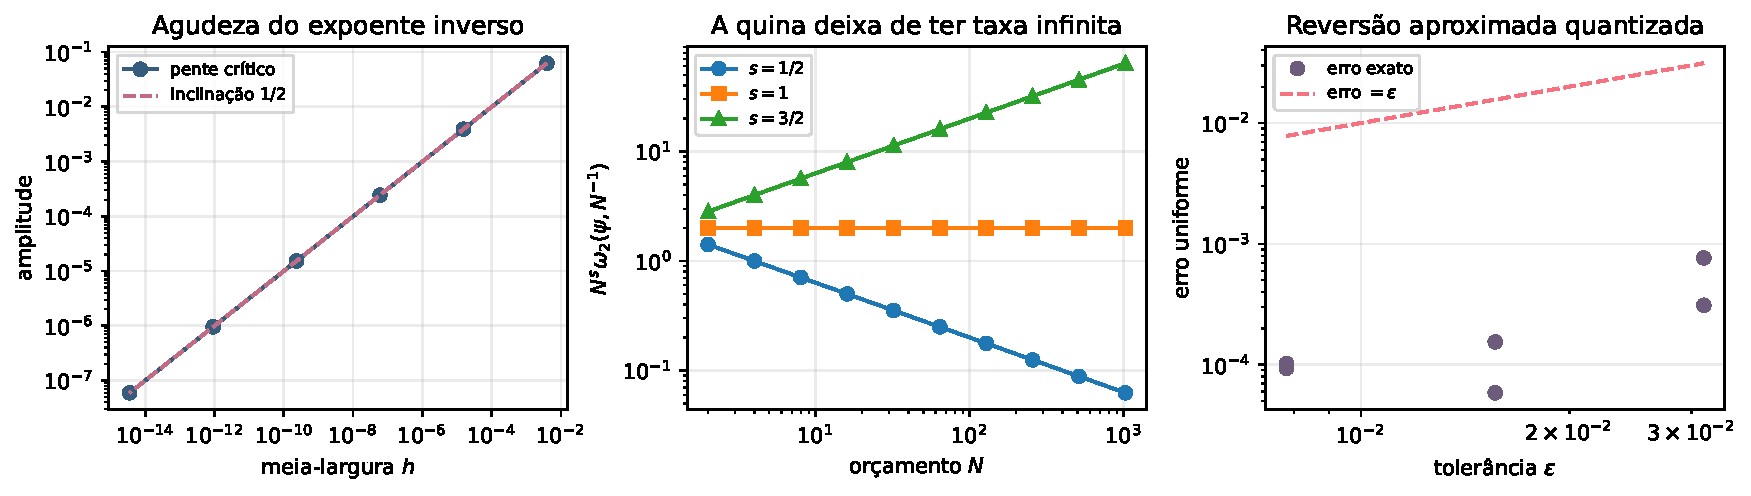
\includegraphics[width=.98\linewidth]{fig_reversibilidade_regularizada.pdf}
 \caption{Três diagnósticos da reversibilidade. À esquerda, o pente de tendas
 realiza o expoente crítico $\alpha/(\alpha+\gamma)$. Ao centro, o certificado
 atribui à quina exatamente a ordem um. À direita, a quantização de redes com
 quebras não diádicas permanece abaixo da tolerância prescrita.}
 \label{fig:regularized-reversibility}
\end{figure}

Os três mecanismos aparecem lado a lado na
\cref{fig:regularized-reversibility}; a coluna relativa ao pente usa agora a
construção na biblioteca original do \cref{thm:critical-tent-comb}.

\subsection{Validação executável}

O programa \texttt{reversibilidade\_regularizada.py} executa uma auditoria
independente em aritmética \texttt{Fraction}. Ele:
\begin{enumerate}[label=(\roman*),leftmargin=2.2em]
 \item executa $2952$ idas e voltas exatas entre formas hinge e árvores
 canônicas, das quais $1160$ contêm ao menos uma região plana;
 \item verifica em todos os casos as duas cotas de folhas de
 \eqref{eq:canonical-tree-leaf-bounds};
 \item quantiza $84$ redes com quebras não diádicas e confere exatamente erro,
 número de folhas, inclinações não nulas e altura;
 \item testa $1260$ instâncias da desigualdade universal que sustenta
 \eqref{eq:universal-regularized-lower};
 \item reproduz a quina em dez escalas, a tenda profunda até $1024$ regiões e
 seis níveis do pente crítico, verificando em cada nível a perturbação, o erro,
 a altura, o número de folhas e a ausência de inclinações nulas na biblioteca
 original.
\end{enumerate}

A reversibilidade assume três formas. A biblioteca $\Library$ corresponde
exatamente à imagem rasa caracterizada por dados racionais, nós diádicos e
inclinações não nulas. A extensão marcada inclui regiões planas e produz uma
bijeção funcional rasa. Redes reais genéricas admitem aproximações inversas
com recursos explícitos. No nível de classes funcionais, o erro bruto possui a recíproca com perda do
\cref{thm:raw-lossy-inverse}, enquanto o certificado
\eqref{eq:self-roughness-certificate} fornece a caracterização direta e
inversa completa do \cref{thm:complete-besov-reversibility}. Essas três formas
separam representação exata, quantização e regularidade funcional.
